


\subsection*{Visualize}


In der Visualisierung soll der Algorithmus für das Layer Assignment durch eine Schritt für Schritt durchführbare Animation dargestellt werden. Die Visualisierung soll voraussichtlich so aussehen:

\begin{figure}[h!]
    \centering
   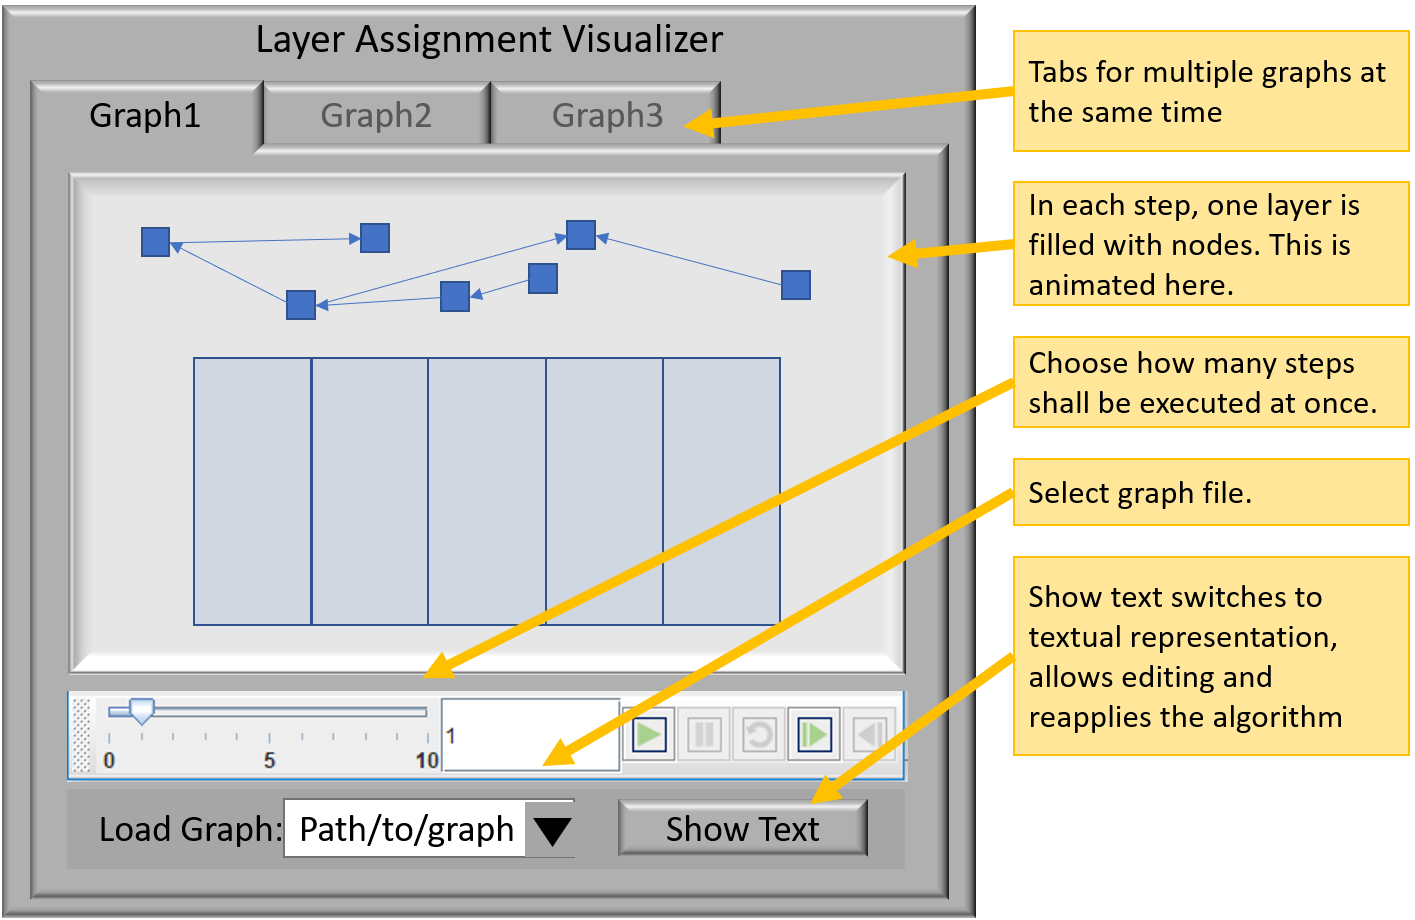
\includegraphics[width=.7\textwidth ]{images/mockupInfo.png}
\end{figure}

Momentan sind noch nicht alle Graphischen Elemente umgesetzt. Die im folgenden Bild grün markierten Bereiche wurden bereits implementiert, sind jedoch teilweise noch nicht mit Funktionalität ausgestattet. Rote Bereiche wurden noch nicht umgesetzt. 
\textbf{Note: Zum testen nur den Step Forwad Knopf verwenden (step size ist einstellebar). Die anderen Knöpfe funktionieren grade nicht oder nicht richtig.}

\begin{figure}[h!]
    \centering
    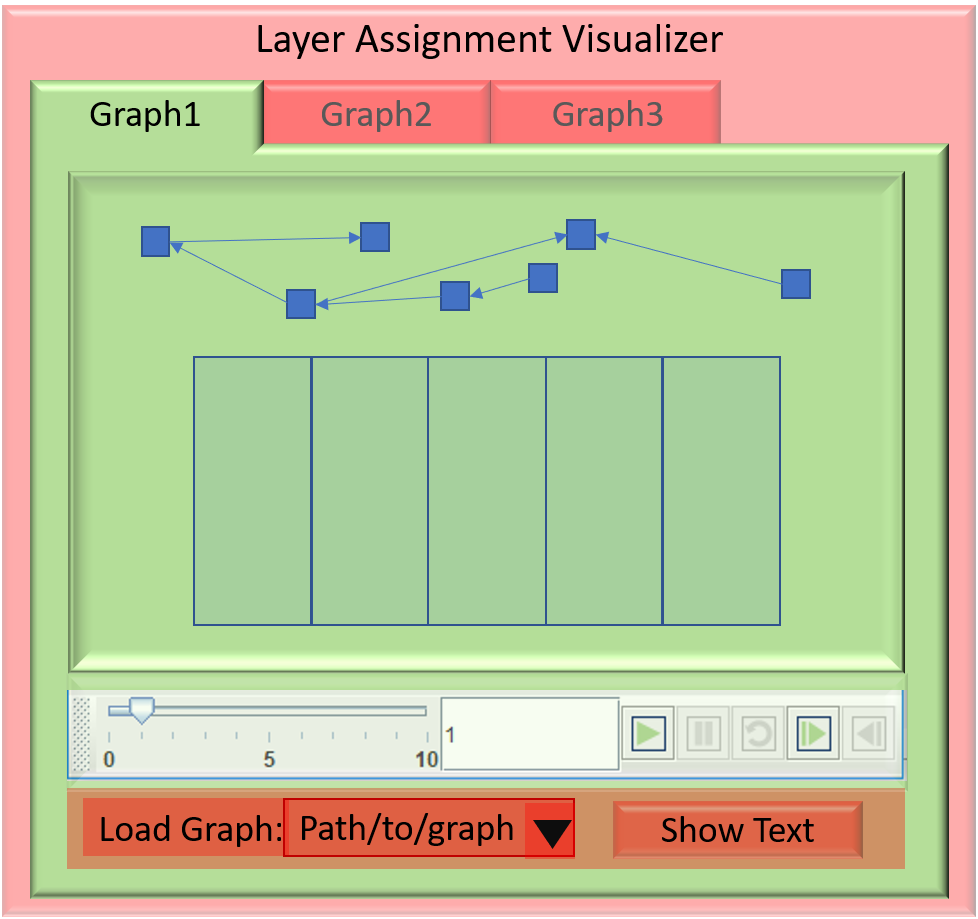
\includegraphics[width=\textwidth / 2]{images/mockupRedGreen.png}
\end{figure}